
\begin{multicols}{2}
Une course internationale de ski de fond
a lieu à Bellin, dans le nord du Québec (70\degres\ Ouest; 60\degres\
Nord) : il s'agit de traverser la baie d'Ungava jusqu'à l'île
Akpatok. Une délégation de skieurs russes s'y rend depuis Leningrad
(30\degres\ Est, 60\degres\ Nord). Leur avion a-t-il intérêt à passer
par le pôle ou bien à suivre le 60\ieme\ parallèle ?
{\em On supposera que le rayon de la Terre est 6\,360~km.}\\
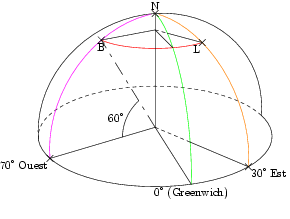
\includegraphics[scale=1]{RepS-48.png} 
\end{multicols}

